\begin{frame}[plain, noframenumbering]
    \begin{center}
        \Huge
        Моделирование гидродинамики методом сглаженных частиц
    \end{center}
\end{frame}

\begin{frame}
    \frametitle{Основные уравнения гидродинамики}

    Уравнения Навье-Стокса для вязкой сжимаемой жидкости
    \begin{itemize}
        \item Уравнение непрерывности:
        \begin{equation}
            \frac{\partial \rho}{\partial t} + \nabla \cdot (\rho \vec{v}) = 0
        \end{equation}
        %
        \item Уравнение импульса:
        \begin{equation}
            \rho \left( \frac{\partial \vec{v}}{\partial t} + \vec{v} \cdot \nabla \vec{v} \right)
                = -\nabla p + \nabla \cdot \tau + \vec{f}
        \end{equation}
        %
        \item Уравнение энергии не используется
        \item Неявный член $\nabla \cdot \tau$ для модели SPH
    \end{itemize}
\end{frame}
\note{
    Этот текст будет виден только если его отображение включено
    в~файле \textbf{Presentation/setup}.
    Для раздельного вывода презентации и заметок на~разные экраны (как
    в~impress или powerpoint) можно использовать программу
    \textit{pdf-presenter-console}.
}

\begin{frame}
    \frametitle{Метод Weakly Compressible SPH}

    Основные идеи метода SPH и его версии WCSPH.

    \begin{itemize}
        \item Аппроксимация функций и производных с помощью сглаживания:
        \begin{equation}\label{eq:sph_approx}
            f(\vec{r}_{i}) = \sum\limits_{j} \frac{m_{j}}{\rho_{j}} f(\vec{r}_{j}) W_{ij}
        \end{equation}
        \begin{equation}
            \nabla\cdot f(\vec{r}_{i}) = \sum\limits_{j} \frac{m_{j}}{\rho_{j}} f(\vec{r}_{j}) \cdot \nabla_{i} W_{ij},
        \end{equation}
        \item Сглаживающее ядро:
        \begin{equation}\label{eq:wendland}
            W = \alpha_{d}
            \begin{cases}
            \begin{tabular}{l l}
                $\left( 1 - \frac{q}{2} \right)^{4} (2q + 1)$
                &
                для $q < 2$
                
                \\
                
                0
                &
                для $q \geq 2$
            \end{tabular}
            \end{cases}
        \end{equation}

        \item Искусственное уравнение состояния:
        \begin{equation}
            p = \frac{c_{0}^{\,2}\rho_{0}}{\gamma}\left( \left( \frac{\rho}{\rho_{0}} \right)^{\gamma} - 1 \right)
        \end{equation}
    \end{itemize}
\end{frame}

\begin{frame}
    \frametitle{Дискретизация уравнений сохранения}
    \begin{itemize}
        \item Уравнение непрерывности:
        \begin{equation}
            \frac{d\rho_{i}}{dt} = \sum\limits_{j}m_{j}\vec{v}_{ij}\cdot\nabla_{i}W_{ij}
        \end{equation}

        \item Уравнение импульса:
        \begin{equation}
            \frac{d\Vec{v}_i}{d t} = -\sum\limits_{j} m_{j} 
                \left(\frac{p_{j}}{\rho_{j}^{2}} + \frac{p_{i}}{\rho_{i}^{2}} + \Pi_{ij} \right) 
                \nabla_{i} W_{ij} + \vec{f}
        \end{equation}

        \item Искусственная вязкость:
        %
        \begin{equation}\label{eq:art_visc}
            \Pi_{ij} = 
            \begin{cases}
            \begin{tabular}{l l}
                $-\displaystyle\frac{\alpha\bar c_{ij}}{\bar\rho_{ij}} \, 
                \left(
                    \frac{h\vec{v}_{ij} \cdot \vec{r}_{ij}}{\vec{r}_{ij}^{\;2} + 0.01h^{2}}
                \right)$ &
                для $\vec{v}_{ij} \cdot \vec{r}_{ij} < 0$, \\
                
                0 &
                для $\vec{v}_{ij} \cdot \vec{r}_{ij} \geq 0$
            \end{tabular}  
            \end{cases}
        \end{equation}
    \end{itemize}
\end{frame}
\note[itemize]{
    \item Тезис 1
    \item Тезис 2
    \item Тезис 3
}

\begin{frame}[plain, noframenumbering]
    \begin{center}
        \Huge
        Реализация ПО для моделирования движения движения жидкости методом SPH
    \end{center}
\end{frame}


\begin{frame}
    \frametitle{Состав разработанного комплекса ПО}
    \begin{itemize}
        \item вычислительные модули:
            \begin{itemize}
                \item \textbf{RRSPH\_CL} --- ускорение с OpenCL
                \item \textbf{RRSPH\_OMP} --- ускорение с OpenMP
            \end{itemize}
        \item модули визуализации:
            \begin{itemize}
                \item \textbf{SPH2D\_Drawer} --- 2D-визуализация
                \item \textbf{Scatter3D} --- 3D-визуализация
            \end{itemize}
        \item аналитический модуль:
            \begin{itemize}
                \item \textbf{FuncAtPoint} --- анализ характеристик поля
                \item \textbf{WaterProfile} --- реконструкция поверхности жидкости
            \end{itemize}
        \item модуль подготовки расчётов:
            \begin{itemize}
                \item \textbf{RRSPH\_GUI} --- интерфейс для настройки параметров модели
                \item скрипты генерации входных данных
                \item скрипт экспорта проектов DualSPHysics
            \end{itemize}
    \end{itemize}
    
\end{frame}
\note[itemize]{
    \item Задача 1
    \item Задача 2
    \item Задача 3
}

\begin{frame}[plain, noframenumbering]
    \begin{center}
        \Huge
        Численные эксперименты и анализ
    \end{center}
\end{frame}

\begin{frame}
    \frametitle{Анализ эффективности}

    \begin{itemize}
        \item Ускорение параллельных вычислений
        \begin{equation}
            S(M) = \frac{T(1)}{T(M)}
        \end{equation}

        \item Эффективность параллельных вычислений
        \begin{equation}
            E(M) = \frac{S(M)}{M}
        \end{equation}
    \end{itemize}


    \bigskip
    \hrule{}
    \bigskip

    Оборудование:
    \begin{itemize}
        \item CPU Intel Core i9-13900F: 8 P-cores + 16 E-cores
        \item GPU NVidia RTX 4070 Ti: 7680 cuda-ядер
    \end{itemize}
\end{frame}

\begin{frame}
    \frametitle{Анализ эффективности. Ускорение}
    \centering{Зависимость ускорения ($S(M) = T(1) / T(M)$) расчёта от количества потоков $M$}
    \center{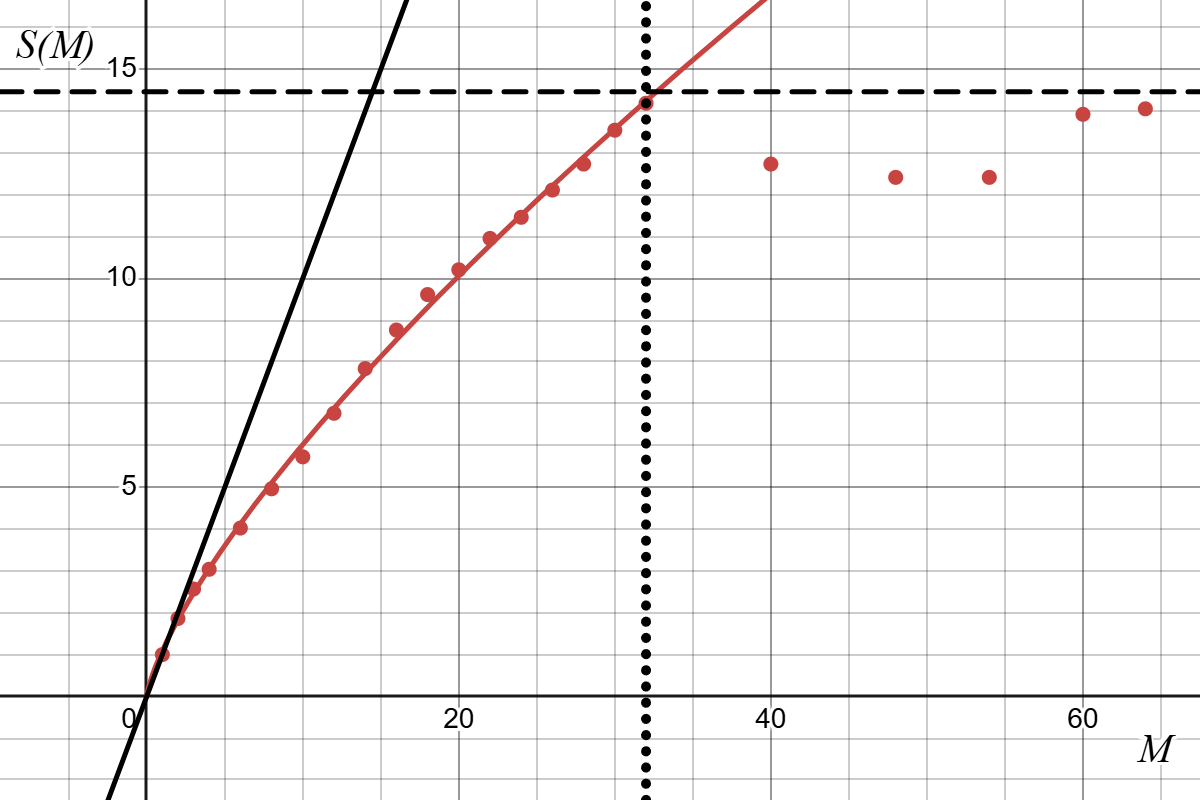
\includegraphics[height=0.75\textheight]{images/Speedup.png}}
\end{frame}

\begin{frame}
    \frametitle{Анализ эффективности. Эффективность}
    \centering{Зависимость эффективности распараллеливания ($E(M) = S(M) / M$) расчёта от количества потоков $M$}
    \center{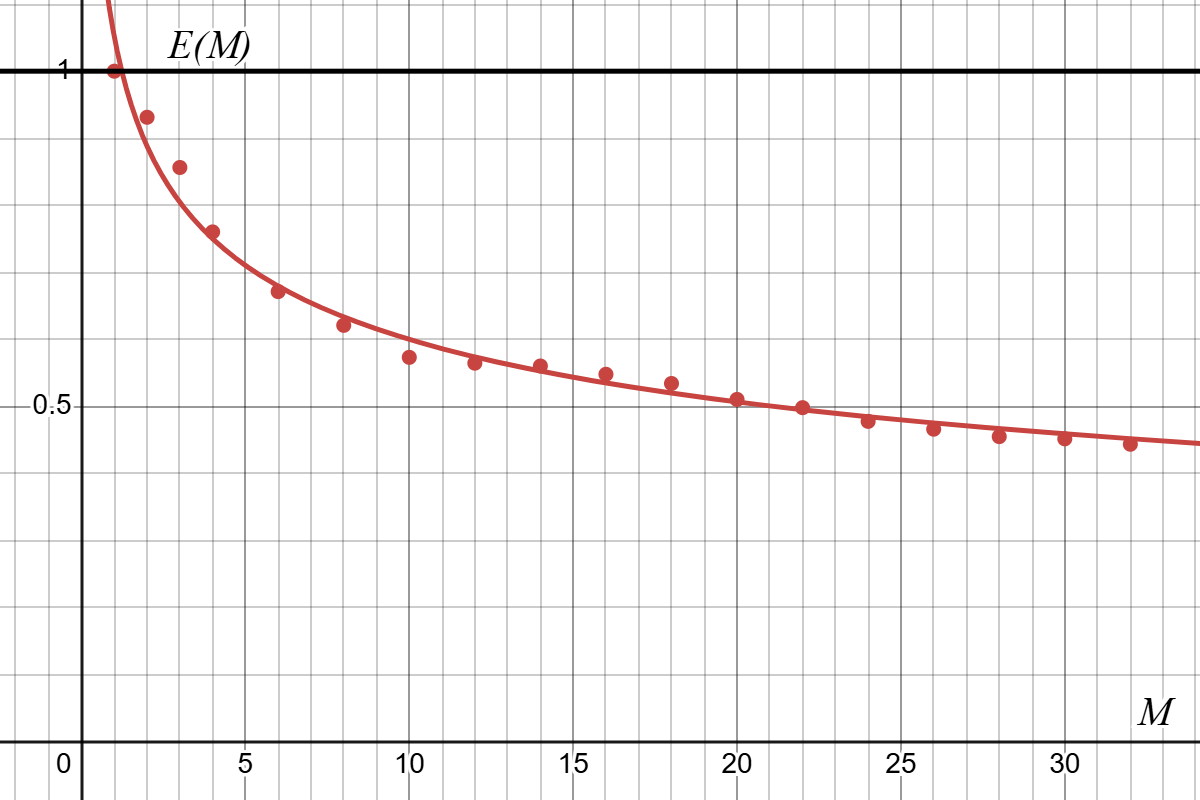
\includegraphics[height=0.75\textheight]{images/Efficiency.png}}
\end{frame}

\begin{frame}
    \frametitle{Анализ эффективности. Результаты}

    \centering
    Ускорение при расчёте 100 шагов по времени различными вычислителями по отношению к однопоточной версии на CPU
    \vfill
    \begin{tabular}{|l|l|l|}
        \hline
        & CPU & GPU \\
        \hline
        float (32 бит) & 11.9 & 23.2 \\
        \hline
        double (64 бит) & 14.5 & 14.1 \\
        \hline
    \end{tabular}

\end{frame}

\begin{frame}
    \frametitle{Расчёт линейных волн. Дисперсионное соотношение}

    \centering
    Ускорение при расчёте 100 шагов по времени различными вычислителями по отношению к однопоточной версии на CPU
    \vfill
    \begin{tabular}{|l|l|l|}
        \hline
        & CPU & GPU \\
        \hline
        float (32 бит) & 11.9 & 23.2 \\
        \hline
        double (64 бит) & 14.5 & 14.1 \\
        \hline
    \end{tabular}

\end{frame}

\begin{frame}
    \frametitle{Векторная графика}
    \begin{figure}
        \centering
        \ifdefmacro{\tikzsetnextfilename}{\tikzsetnextfilename{tikz_presentation}}{}% присваиваемое предкомпилированному pdf имя файла (не обязательно)
        \input{Presentation/images/tikz_plot.tikz}
    \end{figure}
\end{frame}

\subsection{Расположение}

\begin{frame}
    \frametitle{Изображения по-вертикали}
    \centering
    \vfill
    \includegraphics[width=0.8\linewidth,height=0.1\textheight]{latex} \\
    \TeX
    \vfill
    \includegraphics[width=0.8\linewidth,height=0.2\textheight]{latex} \\
    \LaTeX
    \vfill
    \includegraphics[scale=0.2]{latex} \\
    \vfill
\end{frame}


\begin{frame}
    \frametitle{Изображения по-горизонтали}
    \begin{minipage}[t]{0.47\linewidth}
        \textbf{Составная \\ подпись 1}
        \center{\includegraphics[width=1\linewidth]{knuth1}}
    \end{minipage}
    \hfill
    \begin{minipage}[t]{0.47\linewidth}
        \textbf{Составная \\ подпись 2}
        \center{\includegraphics[width=1\linewidth]{knuth2}}
    \end{minipage}
\end{frame}

\subsection{Линии}

\begin{frame}
    \frametitle{Разделяющие линии}
    \begin{minipage}[c]{0.47\linewidth}
        \center{\includegraphics[width=1\linewidth]{latex}}
        \bigskip
        \hrule{}
        \bigskip
        \textbf{Составная \\ подпись 1}
    \end{minipage}
    \hfill
    \vrule{}
    \hfill
    \begin{minipage}[c]{0.47\linewidth}
        \flushright
        \textbf{Составная \\ подпись 2}
        \center{\includegraphics[width=1\linewidth]{knuth2}}
    \end{minipage}
\end{frame}

\section{Остальное}
\begin{frame}[plain, noframenumbering]
    \begin{center}
        \Huge
        Остальное
    \end{center}
\end{frame}

\subsection{Формулы}

\begin{frame}
    \frametitle{Формулы}
    \[
    \left\{
    \begin{array}{rl}
        \dot x = & \sigma (y-x)  \\
        \dot y = & x (r - z) - y \\
        \dot z = & xy - bz
    \end{array}
    \right.
    \]
\end{frame}

\begin{frame}
    \frametitle{amsmath}
    \centering
    \begin{minipage}[t]{0.5\linewidth}
        \begin{multline*}
            y = 1 x^1 + 2 x^2 + 3 x^3 + \\ + 4 x^4 + 5 x^5 + \dots
        \end{multline*}
    \end{minipage}
\end{frame}

\begin{frame}[allowframebreaks]
    \frametitle{Уравнения Максвелла}
    \centering{
        \small
        \def\arraystretch{1.8}%
        \begin{tabular}{ll}
            \toprule
            Интегральная форма                                                                                                                                            & Дифференциальная форма                                                          \\ \midrule
            \(Q_e(t) = \displaystyle\oiint_S \vec D(t) \cdot d\vec{s} = \displaystyle\iiint_V \rho_v(t) dv\)                                                              & \(\nabla \cdot \vec D(t) = \rho_v(t)\)                                          \\
            \(\displaystyle\oiint_S \vec B(t) \cdot d\vec{s} = 0\)                                                                                                        & \(\nabla \cdot \vec B(t) = 0\)                                                  \\
            \(V_{emf}(t) = \displaystyle\oint_L \vec E(t) \cdot d\vec{l}\) = \(- \displaystyle\iint_S \left[\frac{\partial\vec{B}(t)}{\partial t}\right] \cdot d\vec{s}\) & \(\nabla \times \vec E(t) = - \frac{\partial\vec{B}(t)}{\partial t}\)           \\
            \(I(t) = \displaystyle\oint_L \vec H(t) \cdot d\vec{l} = \displaystyle\iint_S \left[\vec J(t) + \frac{\partial\vec{D}(t)}{\partial t}\right] \cdot d\vec{s}\) & \(\nabla \times \vec H(t) = \vec J(t) + \frac{\partial\vec{D}(t)}{\partial t}\) \\ \midrule
            \(\displaystyle\oiint_S \vec J \cdot d\vec{s} = -\frac{\partial Q_e}{\partial t}\)                                                                            & \(\nabla \cdot \vec J = - \frac{\partial \rho_v}{\partial t}\)                  \\
            \bottomrule
            \multicolumn{2}{c}{\(\vec D(t) = \left[\varepsilon(t)\right] * \vec E(t)\)}                                                                                                                                                                     \\
            \multicolumn{2}{c}{\(\vec B(t) = \left[\mu(t)\right] * \vec H(t)\)}                                                                                                                                                                             \\
        \end{tabular}
    }
    \framebreak

    \hspace{0.05\linewidth}
    \centering{
        \small
        \def\arraystretch{1.8}%
        \begin{tabular}{ll}
            \toprule
            Интегральная форма                                                                                                                & Дифференциальная форма                               \\ \midrule
            \(Q_e = \displaystyle\oiint_S \vec D \cdot d\vec{s} = \displaystyle\iiint_V \rho_v dv\)                                           & \(\nabla \cdot \vec D = \rho_v\)                     \\
            \(\displaystyle\oiint_S \vec B \cdot d\vec{s} = 0\)                                                                               & \(\nabla \cdot \vec B = 0\)                          \\
            \(V_{emf} = \displaystyle\oint_L \vec E \cdot d\vec{l}\) = \(- \displaystyle\iint_S \left[j \omega \vec B\right] \cdot d\vec{s}\) & \(\nabla \times \vec E = - j \omega \vec B\)         \\
            \(I = \displaystyle\oint_L \vec H \cdot d\vec{l} = \displaystyle\iint_S \left[\vec J + j \omega \vec D\right] \cdot d\vec{s}\)    & \(\nabla \times \vec H = \vec J + j \omega \vec{D}\) \\ \midrule
            \(\displaystyle\oiint_S \vec J \cdot d\vec{s} = - j \omega Q_e\)                                                                  & \(\nabla \cdot \vec J = - j \omega \rho_v\)          \\
            \bottomrule
            \multicolumn{2}{c}{\(\vec D(t) = \left[\varepsilon\right] \vec E(t)\)}                                                                                                                   \\
            \multicolumn{2}{c}{\(\vec B(t) = \left[\mu\right] \vec H(t)\)}                                                                                                                           \\
        \end{tabular}
    }
\end{frame}

\subsection{Таблицы}

\begin{frame}
    \frametitle{Таблица}
    \centering
    \begin{tabular}{|l|l|}
        \hline
        \textbf{Заголовок 1} & \textbf{Заголовок 2} \\
        \hline
        Сумма                & \(b+a\)              \\
        \hline
        Разность             & \(a-b\)              \\
        \hline
        Произведение         & \(a*b\)              \\
        \hline
    \end{tabular}
\end{frame}

\begin{frame}
    \frametitle{Другая таблица}
    \centering
    \begin{tabular}{lc}
        \toprule
        \multicolumn{1}{c}{\textbf{Заголовок 1}} & \textbf{Заголовок 2} \\ \midrule
        Сумма                                    & \(b+a\)              \\
        Разность                                 & \(a-b\)              \\
        Произведение                             & \(a*b\)              \\
        \bottomrule
    \end{tabular}
\end{frame}


\subsection{Разное}

\begin{frame}
    \frametitle{Большой многоуровневый список}
    \begin{itemize}
        \item \textbf{Пункт 1}
              \begin{itemize}
                  \itemi Подпункт 1-1
                  \itemi Подпункт 1-2
              \end{itemize}
        \item \textbf{Пункт 2}
              \begin{itemize}
                  \itemi Подпункт 2-1
              \end{itemize}
        \item \textbf{Пункт 3}
              \begin{itemize}
                  \itemi Подпункт 3-1
                  \itemi Подпункт 3-2
              \end{itemize}
        \item \textbf{Пункт 4}
              \begin{itemize}
                  \itemi Подпункт 4-1
              \end{itemize}
        \item \textbf{Пункт 5}
              \begin{itemize}
                  \itemi Подпункт 5-1
                  \itemi Подпункт 5-2
                  \itemi Подпункт 5-3
              \end{itemize}
    \end{itemize}
\end{frame}

\begin{frame}
    \frametitle{Четыре изображения}
    \centering
    \includegraphics[width=0.35\linewidth,angle=35]{latex}
    \includegraphics[width=0.35\linewidth,angle=135]{latex}\\
    \includegraphics[width=0.35\linewidth,angle=15]{latex}
    \includegraphics[width=0.35\linewidth,angle=-15]{latex}
\end{frame}

